\documentclass[11pt,notitlepage]{article}
\usepackage[margin=1in]{geometry}
\usepackage{epsfig}
\usepackage{subfigure}
\usepackage{amsmath}
\usepackage[usenames,dvipsnames,svgnames,table]{xcolor}
\usepackage{amssymb}
\usepackage{setspace}
\usepackage{graphicx} % Include figure files
\usepackage{times}
\usepackage{amsthm}
\usepackage[numbers,sort&compress]{natbib}
\usepackage{hyperref}
\hypersetup{bookmarks=true, unicode=false, pdftoolbar=true, pdfmenubar=true, pdffitwindow=false, pdfstartview={FitH}, pdfcreator={}, pdfproducer={}, pdfkeywords={} {} {}, pdfnewwindow=true, colorlinks=true, linkcolor=red, citecolor=Green, filecolor=magenta, urlcolor=cyan,}
\usepackage{authblk}
\usepackage{bbm}
\newtheorem{proposition}{Proposition}
 
\usepackage{parskip}
 
 
\newcommand{\dan}[1]{\textcolor{blue}{#1}}
\newcommand{\vlr}[1]{\textcolor{red}{#1}}

\newcommand{\numpeople}{M}
\newcommand{\numdays}{N}
\newcommand{\samplematrix}{\mathbf{A}}
\newcommand{\samplematrixentry}{A}
\newcommand{\incidence}{c}
\newcommand{\assaycost}{\sigma}

\newcommand{\li}{\ell_i}
\newcommand{\lo}{\ell_0}

\newcommand{\prob}{\mathbb{P}}
\newcommand{\expec}{\mathbb{E}}

 
\begin{document}
%%%%%%%%%% Authors
\author[1]{\vlr{Violet Ross}\thanks{violet.ross@colorado.edu}}
\author[1,2,3]{\dan{Daniel B. Larremore}\thanks{daniel.larremore@colorado.edu}}
\affil[1]{Department of Computer Science, University of Colorado Boulder, Boulder, CO 80309 USA}
\affil[2]{BioFrontiers Institute, University of Colorado Boulder, Boulder, CO 80303 USA}
\affil[3]{Santa Fe Institute, Santa Fe, NM 87501 USA}
%%%%%%%%%% Suppress Date
\date{}
%%%%%%%%%% Title
\title{Title}
\maketitle
%%%%%%%%%% Abstract
\begin{abstract}
abstract
\end{abstract}
%%%%%%%%%% Content


    %%%    
    %%%   
  %%%%%%%
   %%%%%
    %%%
     %

\section{Background}
\label{sec-intro}


Viral kinetics, changes in the concentration of virus within an infected individual over time, were first modeled for the study of HIV in the 1990s \cite{perelson1996hiv}.
Since then, viral kinetics (VK) models have proved useful for a variety of tasks.
VK modeling can be used to address clinical questions, concerning topics like drug resistance \cite{rong2012modeling} and antiviral therapies \cite{heldt2013multiscale}, as well as epidemiological questions, such as understanding trasmissibility over time [CITE] and determining optimal surveillance strategies \cite{kissler2021viral}.  
Modeling viral kinetics also allows us to understand how infections with the same virus might vary depending factors such as the variant \cite{russell2024combined}, the vaccination status of the host \cite{ke2022longitudinal}, whether the host has been infected before \cite{kissler2023viral}, and demographic characteristics of the host, such as age \cite{russell2024combined}.

The fundamental challenge of building VK models is the amount and type of data needed, and the cost associated with collecting it.
If too few samples are collected, the model will struggle to accurately estimate the dynamics of viral concentration, producing poor estimates of epidemiological parameters.
Collecting high numbers of samples presents its own challenges, increasing discomfort for subjects and incurring high costs for the investigator \cite{canini2011viral}. 
Data for fitting VK models may be collected via a challenge study or from naturally occurring infections in some population.
Popular approaches for collecting naturally-occurring infection data, such as serial sampling after an initial positive and aggregating single samples from individuals, produce models with fundamental flaws \cite{russell2024combined}.
Data from challenge studies is often more robust, but is costly to obtain.

Gold-standard data for VK modeling emerged as a result of surveillance efforts during the SARS-CoV-2 pandemic, enabling an influx of VK modeling research which was crucial to improving understanding of the pathogen and making public health decisions [CITE, CITE, CITE].
Existing data that has been collected from as many participants and with as much frequency as the COVID-era data is rare.
We aim to build VK models that are as accurate as those built on the extensive COVID surveillance data — without requiring costly data collection.
Optimal design for VK modeling has been explored in previous work — Canini and Carrat investigated the optimal number of participants, number of samples per participant, and temporal distribution of these samples for fitting a mechanistic model of influenza \cite{canini2011viral}.
We propose an adaptive approach to fitting a generalized phenomonological model of viral kinetics that is optimal with respect to number of assays used.

To optimally identify infections in a population, our approach employs sample pooling. 
Sample pooling was first proposed by Robert Dorfman as a strategy for syphilis screening in the United States military during World War II. 
The limit of detection for many assays is often far lower \vlr{[HOW MUCH]} than the amount of virus in a single positive sample. 
This fact is the basis of sample pooling — combining several samples into a ``pool'' and then testing the pool using a single assay.
If the pool is negative, all of its constituent samples are negative.
If the pool is positive, at least one of the samples within it is positive.
Several approaches optimized for varying criteria have been proposed for determining which of the samples in a positive pool are themselves positive \cite{furstenau2020sample}.
Though Dorfman's design was never employed during the war, it has proved useful since then for providing diagnostic results using less reagant and with a faster turnaround time, as well as reducing the cost associated with obtaining population-level prevelance estimates \cite{grobe2021sample}.

We determine an optimal testing algorithm for a phenomonological viral kinetics model.
This two-phase piecewise linear model with parameters drawn from a Bayesian hierarchical model, has been used to model viral kinetics in work on SARS-CoV-2 \cite{kissler2023viral} and \vlr{other viruses} \cite{}.


\section{Study Design and Optimized Assay Approaches}
We develop methods for fitting a viral kinetics model given a set of \vlr{(is there a word more general than "saliva" that I can use here?)} samples collected from $\numpeople$ individuals over $\numdays$ days.
These samples can be arranged into an $\numpeople$ by $\numdays$ matrix $\samplematrix$, where an entry $\samplematrixentry_{i,j}$ is the sample collected from participant $i$ on day $j$.
We say that $\samplematrixentry_{i,j} > 0$ if individual $i$ had viral RNA concentration above the limit of detection (LOD) of our assay on day $j$.
Otherwise, $\samplematrixentry_{i,j} = 0$. 
Observing the value of an entry in the matrix amounts to assaying the corresponding sample.

Data of this kind might emerge in a variety of ways.
Samples originally collected for a study focusing on one pathogen can be arranged into this format and used to fit a model of another pathogen.
\vlr{(Need another example of where this data might come from.)}
Of course, researchers might collect samples from a population with the express purpose of employing the assaying approaches proposed here.

The ultimate goal of this work is to develop efficient algorithms to obtaining a fit model of the viral kinetics of a pathogen, starting from the matrix $\samplematrix$ whose values we have not yet observed. 
There are two main types of algorithms we propose towards this end: the first locates infections within the sample matrix and the second fits a viral kinetics model to those infections.

Unless researchers specifically target individuals who they know are likely to become infected within a fixed period of time (an approach which incurs its own high expenses), $\samplematrix$ will be a sparse matrix.
If we were to assay every sample in $\samplematrix$, most of the results will be negative, offering little information to our model.
That is, only a small proportion of the assays perfomed in the complete assaying case are informative.
This suggests that we can locate the infections within $\samplematrix$ using far fewer than the $\numpeople * \numdays$ assays required by the complete testing approach.
But how many tests are actually needed, and how should we distribute them among the samples?

\subsection{Sample Pooling and Interval Sampling}
The problem of infection location amounts to identifying continuous sequences of positive entries within the rows of $\samplematrix$.
We need not record the entire infection from start to finish, but rather identify at least one of the positive values within it.
This can be achieved by the following algorithm.

Suppose you are given the matrix $\samplematrix$ with unobserved entries.
Assume that the duration of each infection $\li$ is drawn from some continuous positive distribution with practical lower bound $\lo$ such that $\prob(\li < \lo) < c$ for some small constant $c$.
\vlr{(how are we doing this in sims since we're working in discrete time?)}

The algorithm proceeds as follows. \vlr{(a diagram might be useful for this)}
Within each row: pool the samples and apply a single assay to the pool \vlr{(gotta show that we'll stay above LO)}. 
For each row $i$ on which the assay returns a negative result, set $\samplematrixentry_{i,j} = 0$ for all $i$.
This row does not contain an infection and can now be removed from consideration.
For each row on which the assay returned a positive result, individually assay entries at an interval of 


  \begin{figure}
      \centering 
      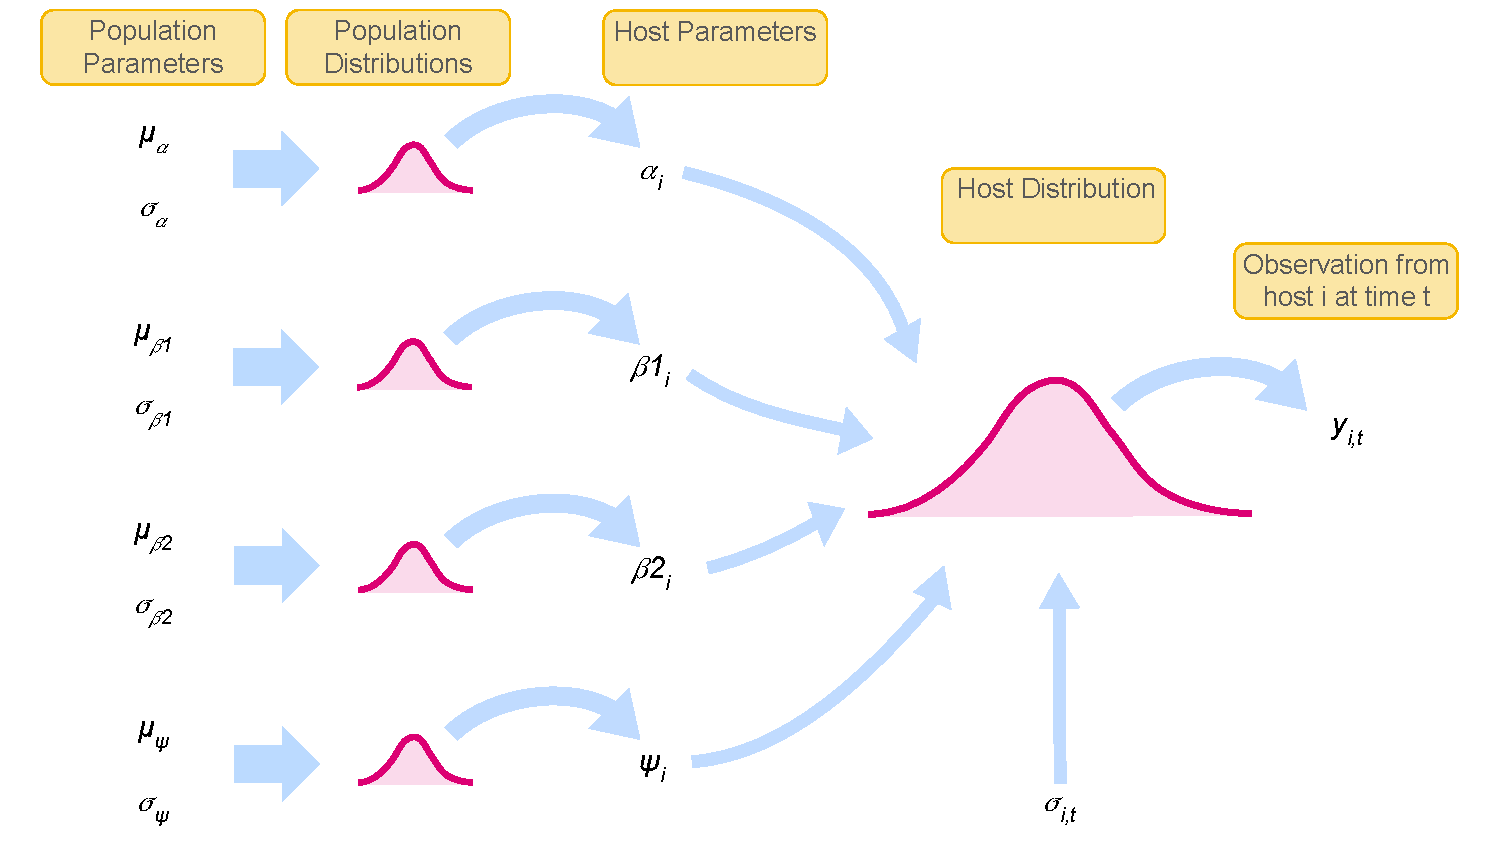
\includegraphics[width=1\textwidth]{../fig/bhm.pdf}
      \caption{The Bayesian hierarchical model.} \label{fig:bhm}
  \end{figure}

  \begin{figure}
      \centering 
      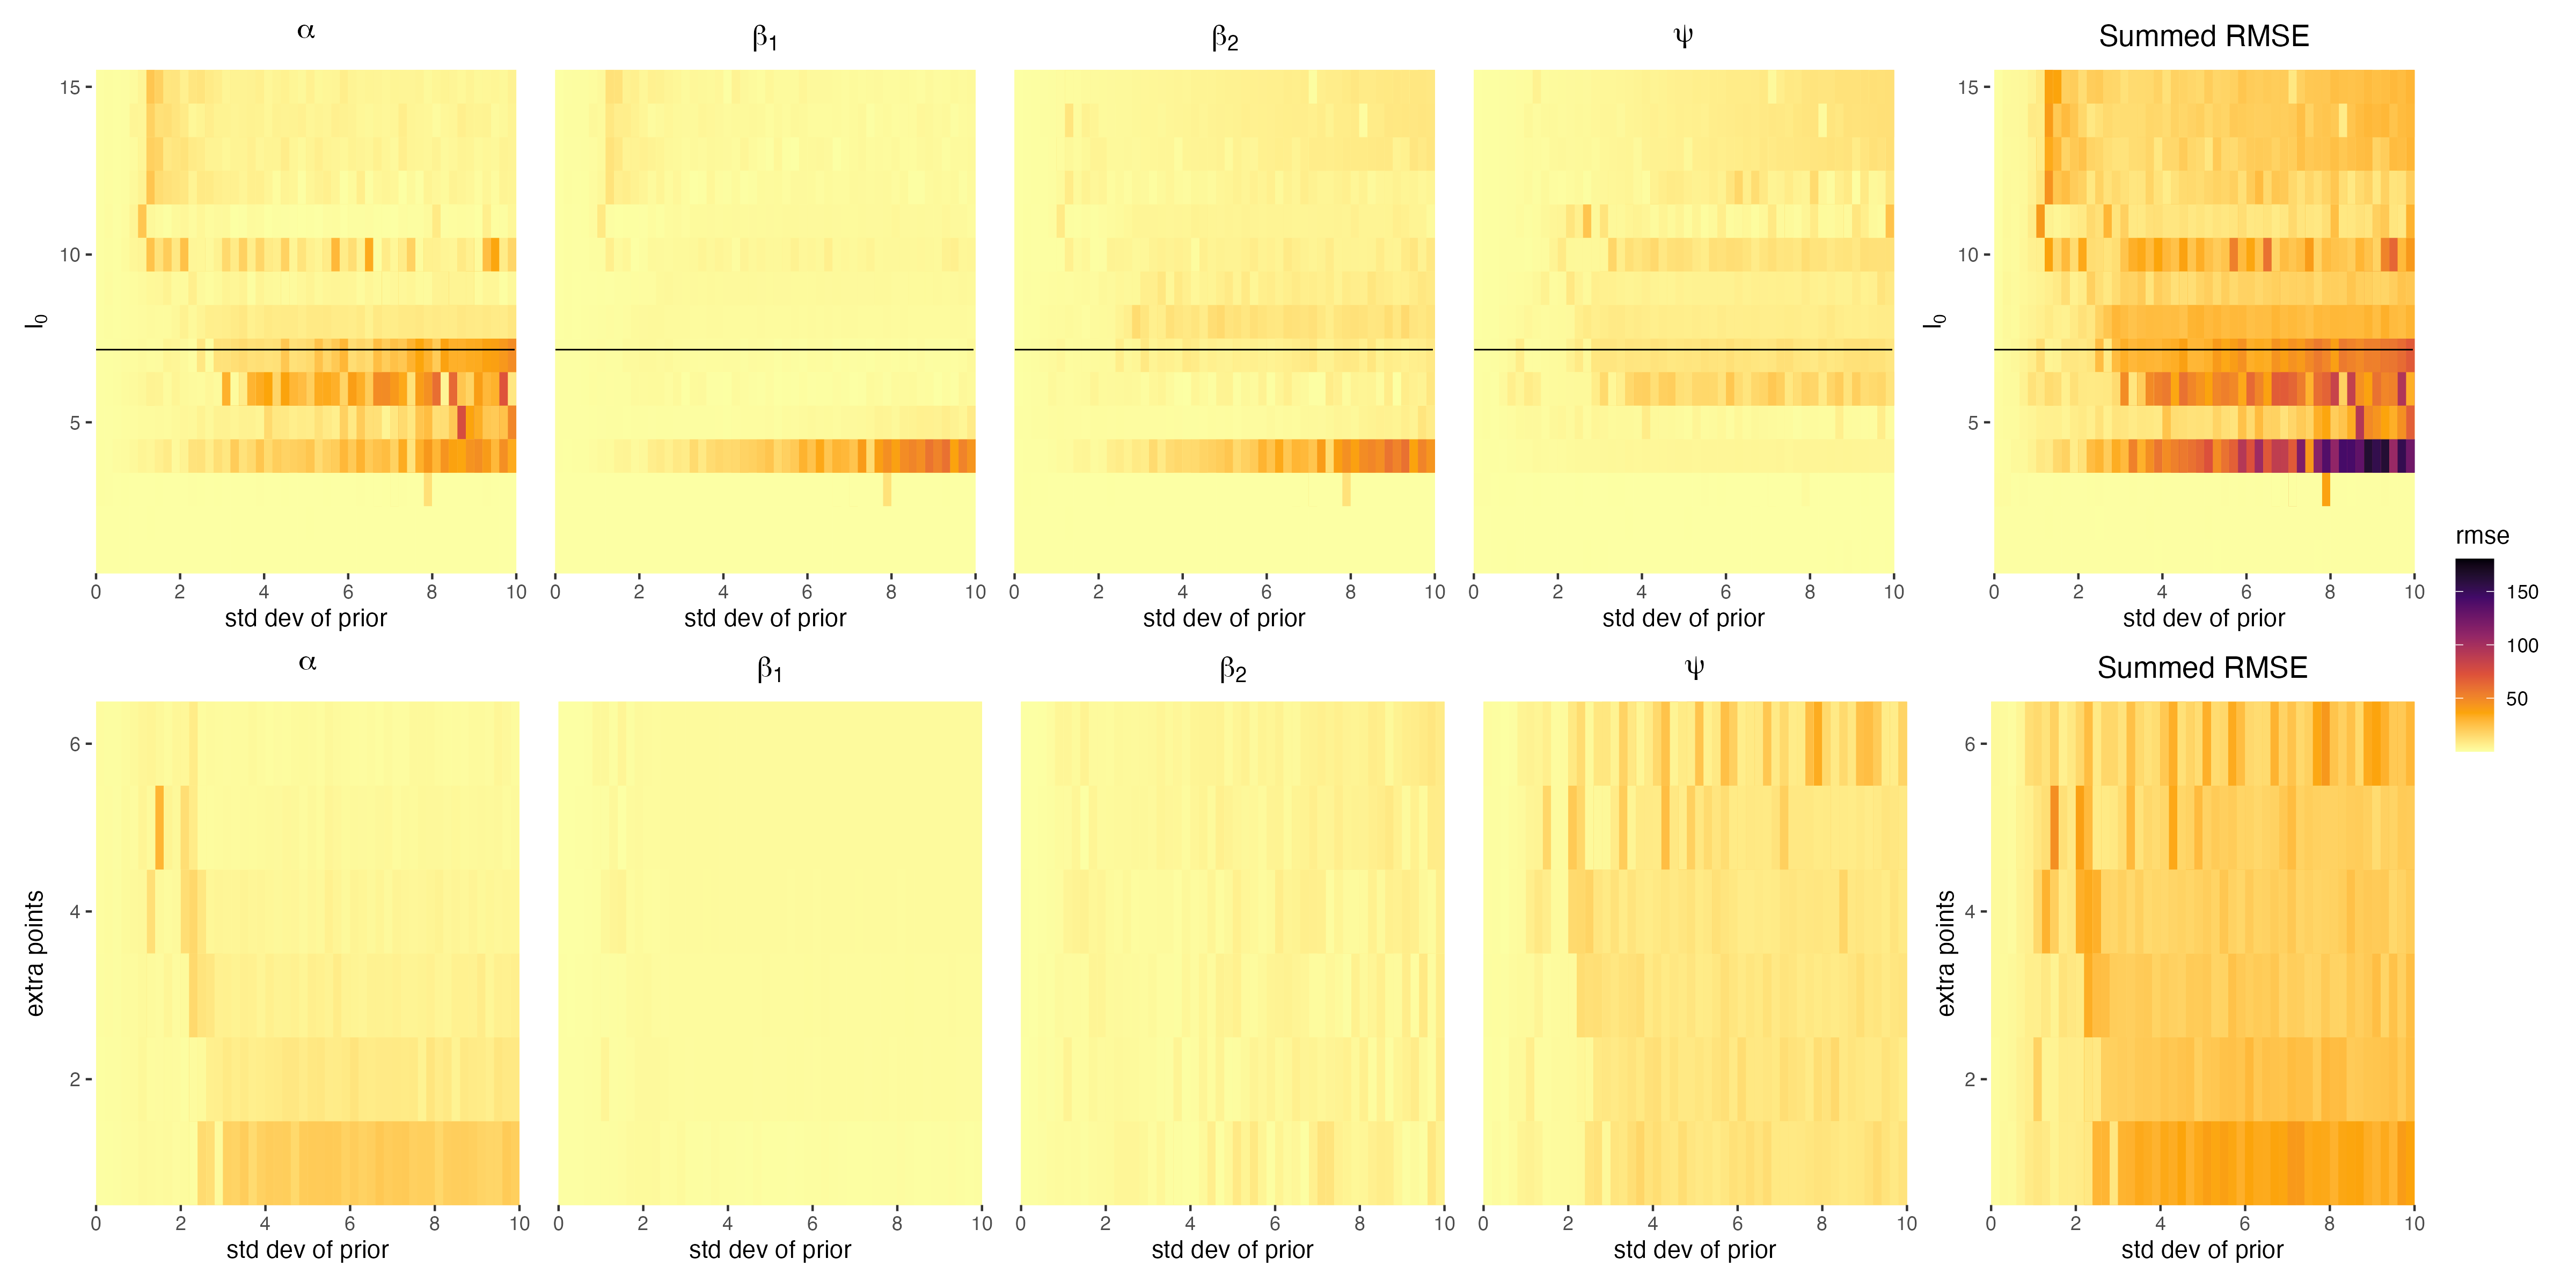
\includegraphics[width=1\textwidth]{../fig/rmse_combined.png}
      \caption{Parameter sweeps.} \label{fig:rmse_combined}
  \end{figure}

  \begin{figure}
      \centering 
      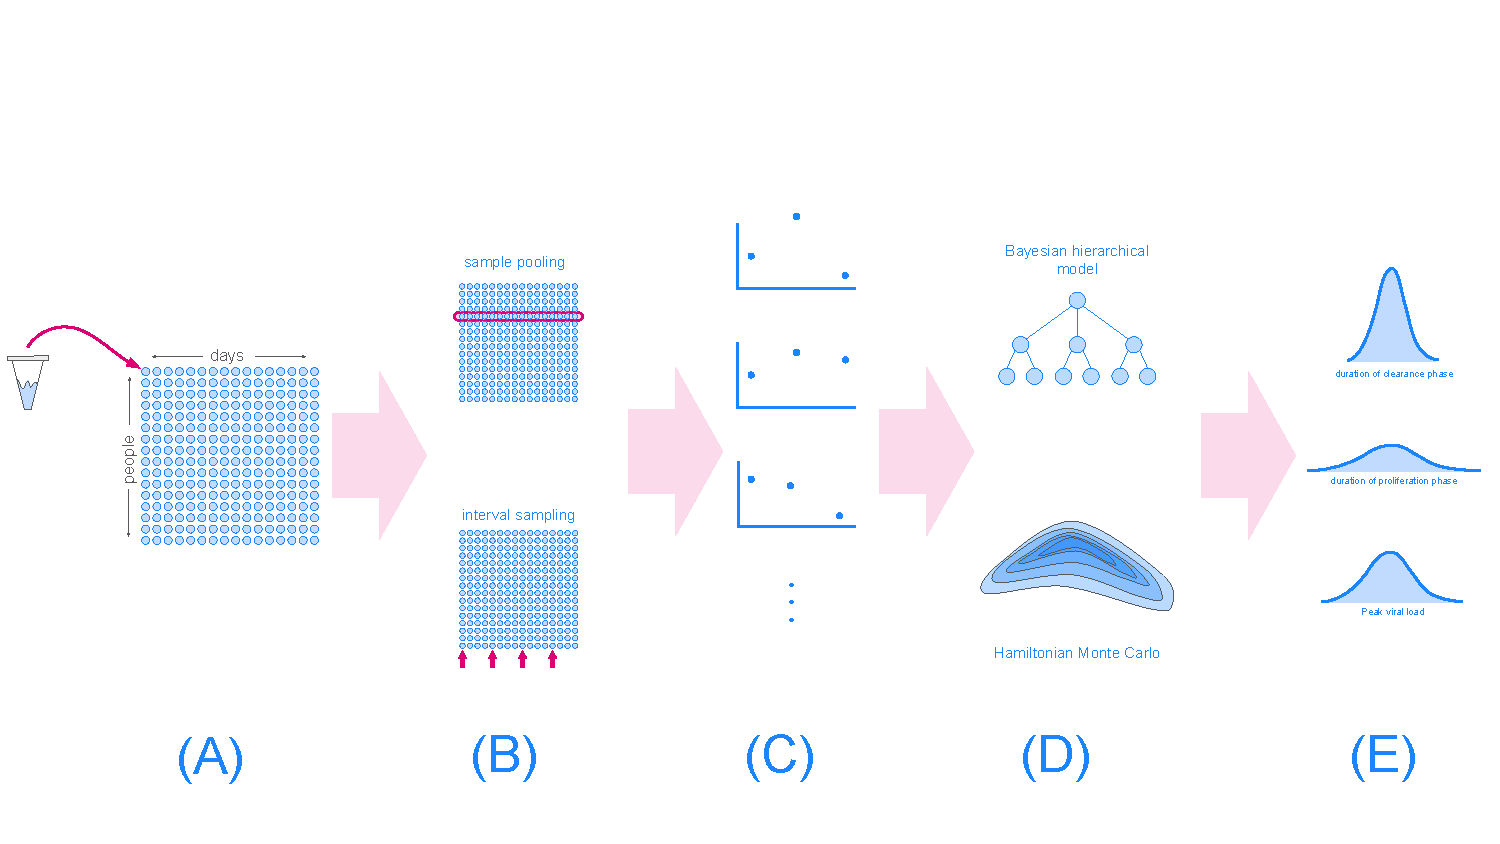
\includegraphics[width=1\textwidth]{../fig/pipeline.pdf}
      \caption{The model fitting pipeline \vlr{(what about adaptive sampling?)}. In Phase (A), subjects provide saliva samples over several
       days to create a matrix of samples with dimensions subjects by days. In Phase (B), sample 
       pooling and interval sampling are used to identify the locations of infections in the 
       matrix. This results in a series of partially sampled viral load trajectories. Using Hamiltonian 
       Monte Carlo, the Bayesian hierarchical model specified in \ref{fig:bhm} is fit to the partially 
       sampled trajectories. The fit model provides probability distributions over possible values of 
       the epidemiological parameters of the pathogen.} \label{fig:pipeline}
       
  \end{figure}

\section{Results}
\subsection{Model Fitting}

\subsection{Interpreting Error}
We have shown that it is possible to reduce the cost of data collection while maintaining the quality of parameter estimates produced by the resulting model.
Still, if some error is permitted, we can reduce costs even further.
It is therefore important for investigators seeking to optimize sample collection and assaying to develop an understanding of how error scales with respect to their question.
To illustrate this, and to contextualize the error values presented in earlier sections of this paper, we provide the following two case studies.
The first case study concerns a question of pathogen dynamics and statistical power, while the second case study concerns an effort to make optimal public health recommendations.

First, suppose we would like to determine whether, for a given pathogen, the peak viral load is different depending on whether the host is vaccinated.
This case study is inspired by the methodologies employed by Kissler et al. in \cite{kissler2023viral}.
We will investigate this question by collecting longitudinal data from two populations: vaccinated and unvaccinated.
This data will be compiled into a matrix onto which our infection discovery algorithm will be applied. 
The trajectories discovered will then be sorted into two groups: V (vaccinated) and U (unvaccinated).
We will separately fit the BHM to group V and group U, skipping any additional point acquisition.
Then, to determine whether the peak viral loads are significantly different, we will take the difference of the two groups' relevant posterior draws entry-wise.
If less than 5\% of the differences fall on a given side of 0, the peaks of the two groups are considered significantly different.

To investiate the impact of reduced assay rate on an investigator's ability to answer the proposed question, we conducted the following experiment.
We generated a synthetic matrix of infections, where the vaccination status of an individual is determined randomly.
There are two separate models from which we generate the viral kinetics for vaccinated and unvaccinated individuals.
The two models are identical except for the distributions from which peak viral load is drawn, which have different means.
If we assay every sample in the matrix, we can correctly determine that the two groups have different underlying peak viral load distributions.

\begin{figure}
    \centering 
    \includegraphics[width=1\textwidth]{../fig/question1.png}
    \caption{Case Study 1.} \label{fig:question1}
\end{figure}


Figure \ref{fig:question1} demonstrates how our ability to identify this difference varies with the interval at which we assay participants.
The complete details of this simulation are available in Appendix [BLAH].
Notably, for values of $\lo$ less than or equal to 6, we are able to correctly detect the difference in the peak viral load distributions of the two groups.
That is, with $1/6$ as many assays, the two groups can still be distinguished.
We also plot the $\beta_1$ RMSE of the two fit models for varying $\lo$.
For some higher $\lo$ values for which the viral load question is correctly answered, the RMSE of the actual parameter estimates are nontrivial.
Therefore, if one wanted to both determine whether unvaccinated and vaccinated populations have significantly different peak viral loads \textit{and} provide accurate estimates of what those peak viral loads are, it would be advantageous to select a smaller sampling interval.
We note, however, that this interval length need not be 1; for $\lo = 3$, the RMSEs of both the model fit to U and the model fit to V are similar to the RMSEs acheived with complete assaying.

This simulation demonstrates that key pathogen kinetics questions can be answered even when the parameter estimates are noisy.
This fact allows for a more extensive reduction in the cost of data collection.
Still, for those questions that require more accurate estimates of epidemiological parameters, costs can be reduced (in this case, by a factor of 3), without sacrificing performance.

In the second case study, we consider the task of selecting the optimal length of isolation for individuals infected with a given pathogen.
To select isolation length, we optimize over testing effectiveness (TE) as defined by Middleton et al. in \cite{BLAH}.
Details on the calculation of TE and the optimization process can be found in Appendix [BLAH].
The value of TE is computed using, among other information, a model of the viral kinetics of the pathogen.

\begin{figure}
    \centering 
    \includegraphics[width=1\textwidth]{../fig/question2.png}
    \caption{Case Study 2.} \label{fig:question2}
\end{figure}

Figure \ref{fig:question2} shows the selected optimal length of isolation for varying amounts of error on the parameter which describes the mean of the clearance phase duration.
This figure highlights the impact of the sign of the error on the isolation recommendation.
Negative error leads to isolation recommendations that are shorter than the true optimal, while positive error generates longer recommended lengths.
Additionally, a lesser magnitude of negative signed error is necessary to alter the recomended length than of positive error.
This brings a key dimension of cost optimization to light — two sampling approaches that cause the same magnitude of error on the parameter estimates, but in opposite directions, may not have the same impact on the researcher's ability to answer their question.
Just as the sign of the error on the clearance phase duration parameter causes varying impacts on the recommended isolation length, the direction in which we erroneously estimate optimal isolation length causes varying public health impacts.
An isolation period that is too short will allow individuals who are still infectious to exit isolation too early, while a longer-than-necessary isolation period may result in an unecessary burden on the infected individual.
Public health officials therefore may allow assaying optimization that biases estimates in one direction, but not the other.

Of course, in the above case studies, we know the correct answer in advance, and can evaluate the performance of optimization efforts by determining whether the undersampled data produces the same result.
When collecting data with the goal of answering a novel question, the researcher must determine the sensitivity of their analysis process to parameter estimate error in advance.

\section{Appendix}

\subsection{Accuracy and Cost of Infection Discovery}\label{sec:infx-disc}
For an arbitrary infection $i$ contained in sample matrix $\samplematrix$, the probability the infection discovery algorithm misses $i$ can be expressed as follows.
\begin{equation*}
    \begin{split}
            \prob(\text{miss }i) &= \prob(\li \geq \lo) \prob(\text{miss }i | \li \geq \lo) + \prob(\li < \lo) \prob(\text{miss }i | \li < \lo) \\
            &= \prob(\li < \lo) \prob(\text{miss }i | \li < \lo) \\
            &= \int_{0}^{\lo} \prob(\li) \prob(\text{miss }i | \li) d\li \\
            &= \int_{0}^{\lo} \prob(\li) \left(1 - \frac{\li}{\lo} \right) d\li  \\
            &= \int_{0}^{\lo} \prob(\li) - \int_{0}^{\lo} \prob(\li)\frac{\li}{\lo} d\li  \\
            &= \prob(\li < \lo) - \frac{\prob(\li < \lo)}{\lo} \expec \left[ \li | \li < \lo \right] \\
            &< \alpha - \frac{\alpha}{\lo} \expec \left[ \li | \li < \lo \right]
    \end{split}
\end{equation*}

We now consider the cost of performing infection discovery on $\samplematrix$.
Suppose each assay costs $\assaycost$.
Then the cost of the pooling step of the infection discovery algorithm is $\assaycost \numpeople$.
The cost of the interval sampling step is 

\bibliographystyle{unsrtnat}
\bibliography{refs}
\end{document}